%
% This is the LaTeX template file for lecture notes for EE 382C/EE 361C.
%
% To familiarize yourself with this template, the body contains
% some examples of its use.  Look them over.  Then you can
% run LaTeX on this file.  After you have LaTeXed this file then
% you can look over the result either by printing it out with
% dvips or using xdvi.
%
% This template is based on the template for Prof. Sinclair's CS 270.

\documentclass[twoside]{article}
\usepackage{graphicx}
\usepackage{hyperref}
\usepackage{algorithm}
\usepackage{algpseudocode}
\usepackage{listings}
%\lstdefinestyle{customc}{
%  belowcaptionskip=1\baselineskip,
%  breaklines=true,
%  frame=L,
%  xleftmargin=\parindent,
%  language=C,
%  showstringspaces=false,
%  basicstyle=\footnotesize\ttfamily,
%  keywordstyle=\bfseries\color{green!40!black},
%  commentstyle=\itshape\color{purple!40!black},
%  identifierstyle=\color{blue},
%  stringstyle=\color{orange},
%}
%
%\lstdefinestyle{customasm}{
%  belowcaptionskip=1\baselineskip,
%  frame=L,
%  xleftmargin=\parindent,
%  language=[x86masm]Assembler,
%  basicstyle=\footnotesize\ttfamily,
%  commentstyle=\itshape\color{purple!40!black},
%}

%\lstset{escapechar=@,style=customc}
\setlength{\oddsidemargin}{0.25 in}
\setlength{\evensidemargin}{-0.25 in}
\setlength{\topmargin}{-0.6 in}
\setlength{\textwidth}{6.5 in}
\setlength{\textheight}{8.5 in}
\setlength{\headsep}{0.75 in}
\setlength{\parindent}{0 in}
\setlength{\parskip}{0.1 in}

%
% The following commands set up the lecnum (lecture number)
% counter and make various numbering schemes work relative
% to the lecture number.
%
\newcounter{lecnum}
\renewcommand{\thepage}{\thelecnum-\arabic{page}}
\renewcommand{\thesection}{\thelecnum.\arabic{section}}
\renewcommand{\theequation}{\thelecnum.\arabic{equation}}
\renewcommand{\thefigure}{\thelecnum.\arabic{figure}}
\renewcommand{\thetable}{\thelecnum.\arabic{table}}

%
% The following macro is used to generate the header.
%
\newcommand{\lecture}[4]{
   \pagestyle{myheadings}
   \thispagestyle{plain}
   \newpage
   \setcounter{lecnum}{#1}
   \setcounter{page}{1}
   \noindent
   \begin{center}
   \framebox{
      \vbox{\vspace{2mm}
    \hbox to 6.28in { {\bf EE 382C/361C: Multicore Computing
                        \hfill Fall 2016} }
       \vspace{4mm}
       \hbox to 6.28in { {\Large \hfill Lecture #1: #2  \hfill} }
       \vspace{2mm}
       \hbox to 6.28in { {\it Lecturer: #3 \hfill Scribe: #4} }
      \vspace{2mm}}
   }
   \end{center}
   \markboth{Lecture #1: #2}{Lecture #1: #2}
   %{\bf Disclaimer}: {\it These notes have not been subjected to the
   %usual scrutiny reserved for formal publications.  They may be distributed
   %outside this class only with the permission of the Instructor.}
   \vspace*{4mm}
}

%
% Convention for citations is authors' initials followed by the year.
% For example, to cite a paper by Leighton and Maggs you would type
% \cite{LM89}, and to cite a paper by Strassen you would type \cite{S69}.
% (To avoid bibliography problems, for now we redefine the \cite command.)
% Also commands that create a suitable format for the reference list.
\renewcommand{\cite}[1]{[#1]}
\def\beginrefs{\begin{list}%
        {[\arabic{equation}]}{\usecounter{equation}
         \setlength{\leftmargin}{2.0truecm}\setlength{\labelsep}{0.4truecm}%
         \setlength{\labelwidth}{1.6truecm}}}
\def\endrefs{\end{list}}
\def\bibentry#1{\item[\hbox{[#1]}]}

%Use this command for a figure; it puts a figure in wherever you want it.
%usage: \fig{NUMBER}{SPACE-IN-INCHES}{CAPTION}
\newcommand{\fig}[3]{
			\vspace{#2}
			\begin{center}
			Figure \thelecnum.#1:~#3
			\end{center}
	}
% Use these for theorems, lemmas, proofs, etc.
\newtheorem{theorem}{Theorem}[lecnum]
\newtheorem{lemma}[theorem]{Lemma}
\newtheorem{proposition}[theorem]{Proposition}
\newtheorem{claim}[theorem]{Claim}
\newtheorem{corollary}[theorem]{Corollary}
\newtheorem{definition}[theorem]{Definition}
\newenvironment{proof}{{\bf Proof:}}{\hfill\rule{2mm}{2mm}}

% **** IF YOU WANT TO DEFINE ADDITIONAL MACROS FOR YOURSELF, PUT THEM HERE:

\begin{document}
%FILL IN THE RIGHT INFO.
%\lecture{**LECTURE-NUMBER**}{**DATE**}{**LECTURER**}{**SCRIBE**}
\lecture{1}{August 24}{Vijay Garg}{Michael Bartling}
%\footnotetext{These notes are partially based on those of Nigel Mansell.}

% **** YOUR NOTES GO HERE:

% Some general latex examples and examples making use of the
% macros follow.  
%**** IN GENERAL, BE BRIEF. LONG SCRIBE NOTES, NO MATTER HOW WELL WRITTEN,
%**** ARE NEVER READ BY ANYBODY.
\section{Introduction}
In this class we introduce the concept of concurrent programming using multiple libraries including Thread programming in Java, pthreads in C, openMP, and CUDA (for GPU compute). We also introduce the concept of formal verification of parallel programming. Finally, we end with an example of a set of parallel forms of a simple algorithm. 

\section{Special Note}

Dr. Garg\'s office hours are a gun free zone. 

\section{Parallel Frameworks}

\textbf{Note:} all of the following code examples can be found at the course GitHub \url{https://github.com/mbartling/UT-Garg-EE382C-EE361C-Multicore/tree/master/chapter1-threads}

\subsection{Java}
Parallelism in Java can be achieved in one of a few ways. In the first method we just extend the Java Thread class:
\lstinputlisting[language=Java]{HelloWorldThread.java}

Another option is to implement \texttt{Run()} such as:
\lstinputlisting[language=Java]{FooBar.java}

\subsection{OpenMP}
OpenMP makes trivial parallel paradigms in C, such as parallel for loops and simple threads, well \textit{trivial}. The following code snippet shows a simple task creation, however parallel for loops are about as simple as \texttt{parfor} in Matlab. In GCC on Linux you need to use the \texttt{-fopenmp} flag to compile with openMP support.

\lstinputlisting[language=C]{helloOpenMP.c}

\subsection{pthreads}
POSIX threads or \textit{pthreads} for short, are a type of thread compatible with the POSIX standard. pthreads are most commonly programmed in C and C++, however they are available in other languages. Furthermore, pthreads are approximately compatible with most common operating systems. Note, in GCC you need to link against the pthreads library to use them, this can be done with the \texttt{-lpthread} linker flag.

\lstinputlisting[language=C]{helloPthread.c}

\subsection{GPGPU's and CUDA Programming}
Traditionally, GPU programming has been \textit{locked in} to graphics oriented tasks. Over time this programming model has shifted towards a more software defined model. Nowadays, GPGPU's, or general purpose graphics processing units, handle many highly parallelizable tasks such as computing the back-propagation algorithm in Deep Neural Networks, Hogwild gradient descent methods, recursive and iterative ray-tracing, and other performance critical parallel computations. The basic programming paradigm is the \textit{kernel}. The kernel describes both a task and how to distribute this task on the GPU including the resources to utilize. Optimizing the kernel is challenging both for programmers and for compiler writers. 

\textbf{NOTE:} CUDA programs can be compiled using \texttt{nvcc}.

\begin{figure}[thbp]
  \centering
  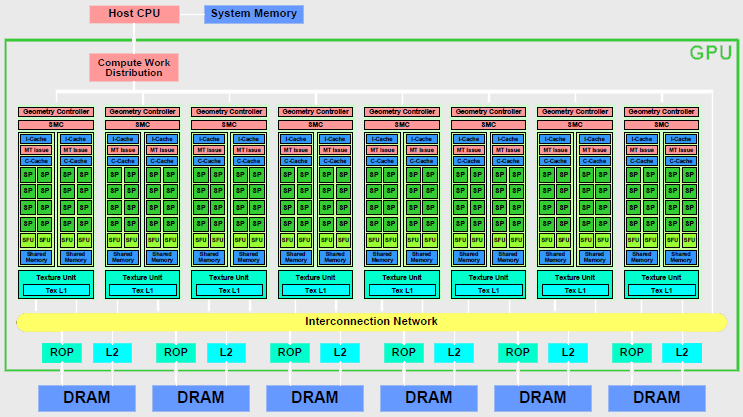
\includegraphics[width=0.95\textwidth]{host-to-gpu}
  \caption{GPU Architecture: GPU's are effectively a multicore processor where each \textit{core} (approximately 15-20) has its own set of compute units. These compute units are often confused with cores in the whitepapers (e.g. the Nvidia GTX 980 has 2200 CUDA cores!). The true cores are often referred to as Streaming Multiprocessors.}
\end{figure}

\begin{lstlisting}
#include <stdio.h>

#define NUM_BLOCKS 16
#define BLOCK_WIDTH 1

__global__ void hello()
{
    printf("Hello world! I'm a thread in block %d\n", blockIdx.x);
}


int main(int argc,char **argv)
{
    // launch the kernel
    hello<<<NUM_BLOCKS, BLOCK_WIDTH>>>();

    // force the printf()s to flush
    cudaDeviceSynchronize();

    printf("That's all!\n");

    return 0;
}
\end{lstlisting}

\section{Formal Verification}
Oftentimes, determining whether our concurrent model is correct is a non-trivial task. Luckily tools like Promela and Spin exist to formally verify our concurrent model. Spin is used to run promela files and is invoked as following 

\texttt{\$> spin promelaFile.pml}

The following is an example of a Promela model:
\begin{lstlisting}
active [2] proctype user()
{
    printf("Hello from thread %d\n", _pid);
}

init {
    printf("Main: Hello from thread %d\n", _pid);
}
\end{lstlisting}

\section{Ideal Parallel RAM model: PRAM}
We can think of PRAM as an "Ideal Parallel Machine," where each processing element, PE, communicates with a shared memory structure. See \ref{fig:pram}. This model is accessed using multiple methods including:

\begin{itemize}
  \item CREW
  \item EREW
  \item Common CRCW
\end{itemize}

Where E stands for exclusive, R for read, W for write, and C for concurrent.

\begin{figure}[thb]
  \label{fig:pram}
  \centering
  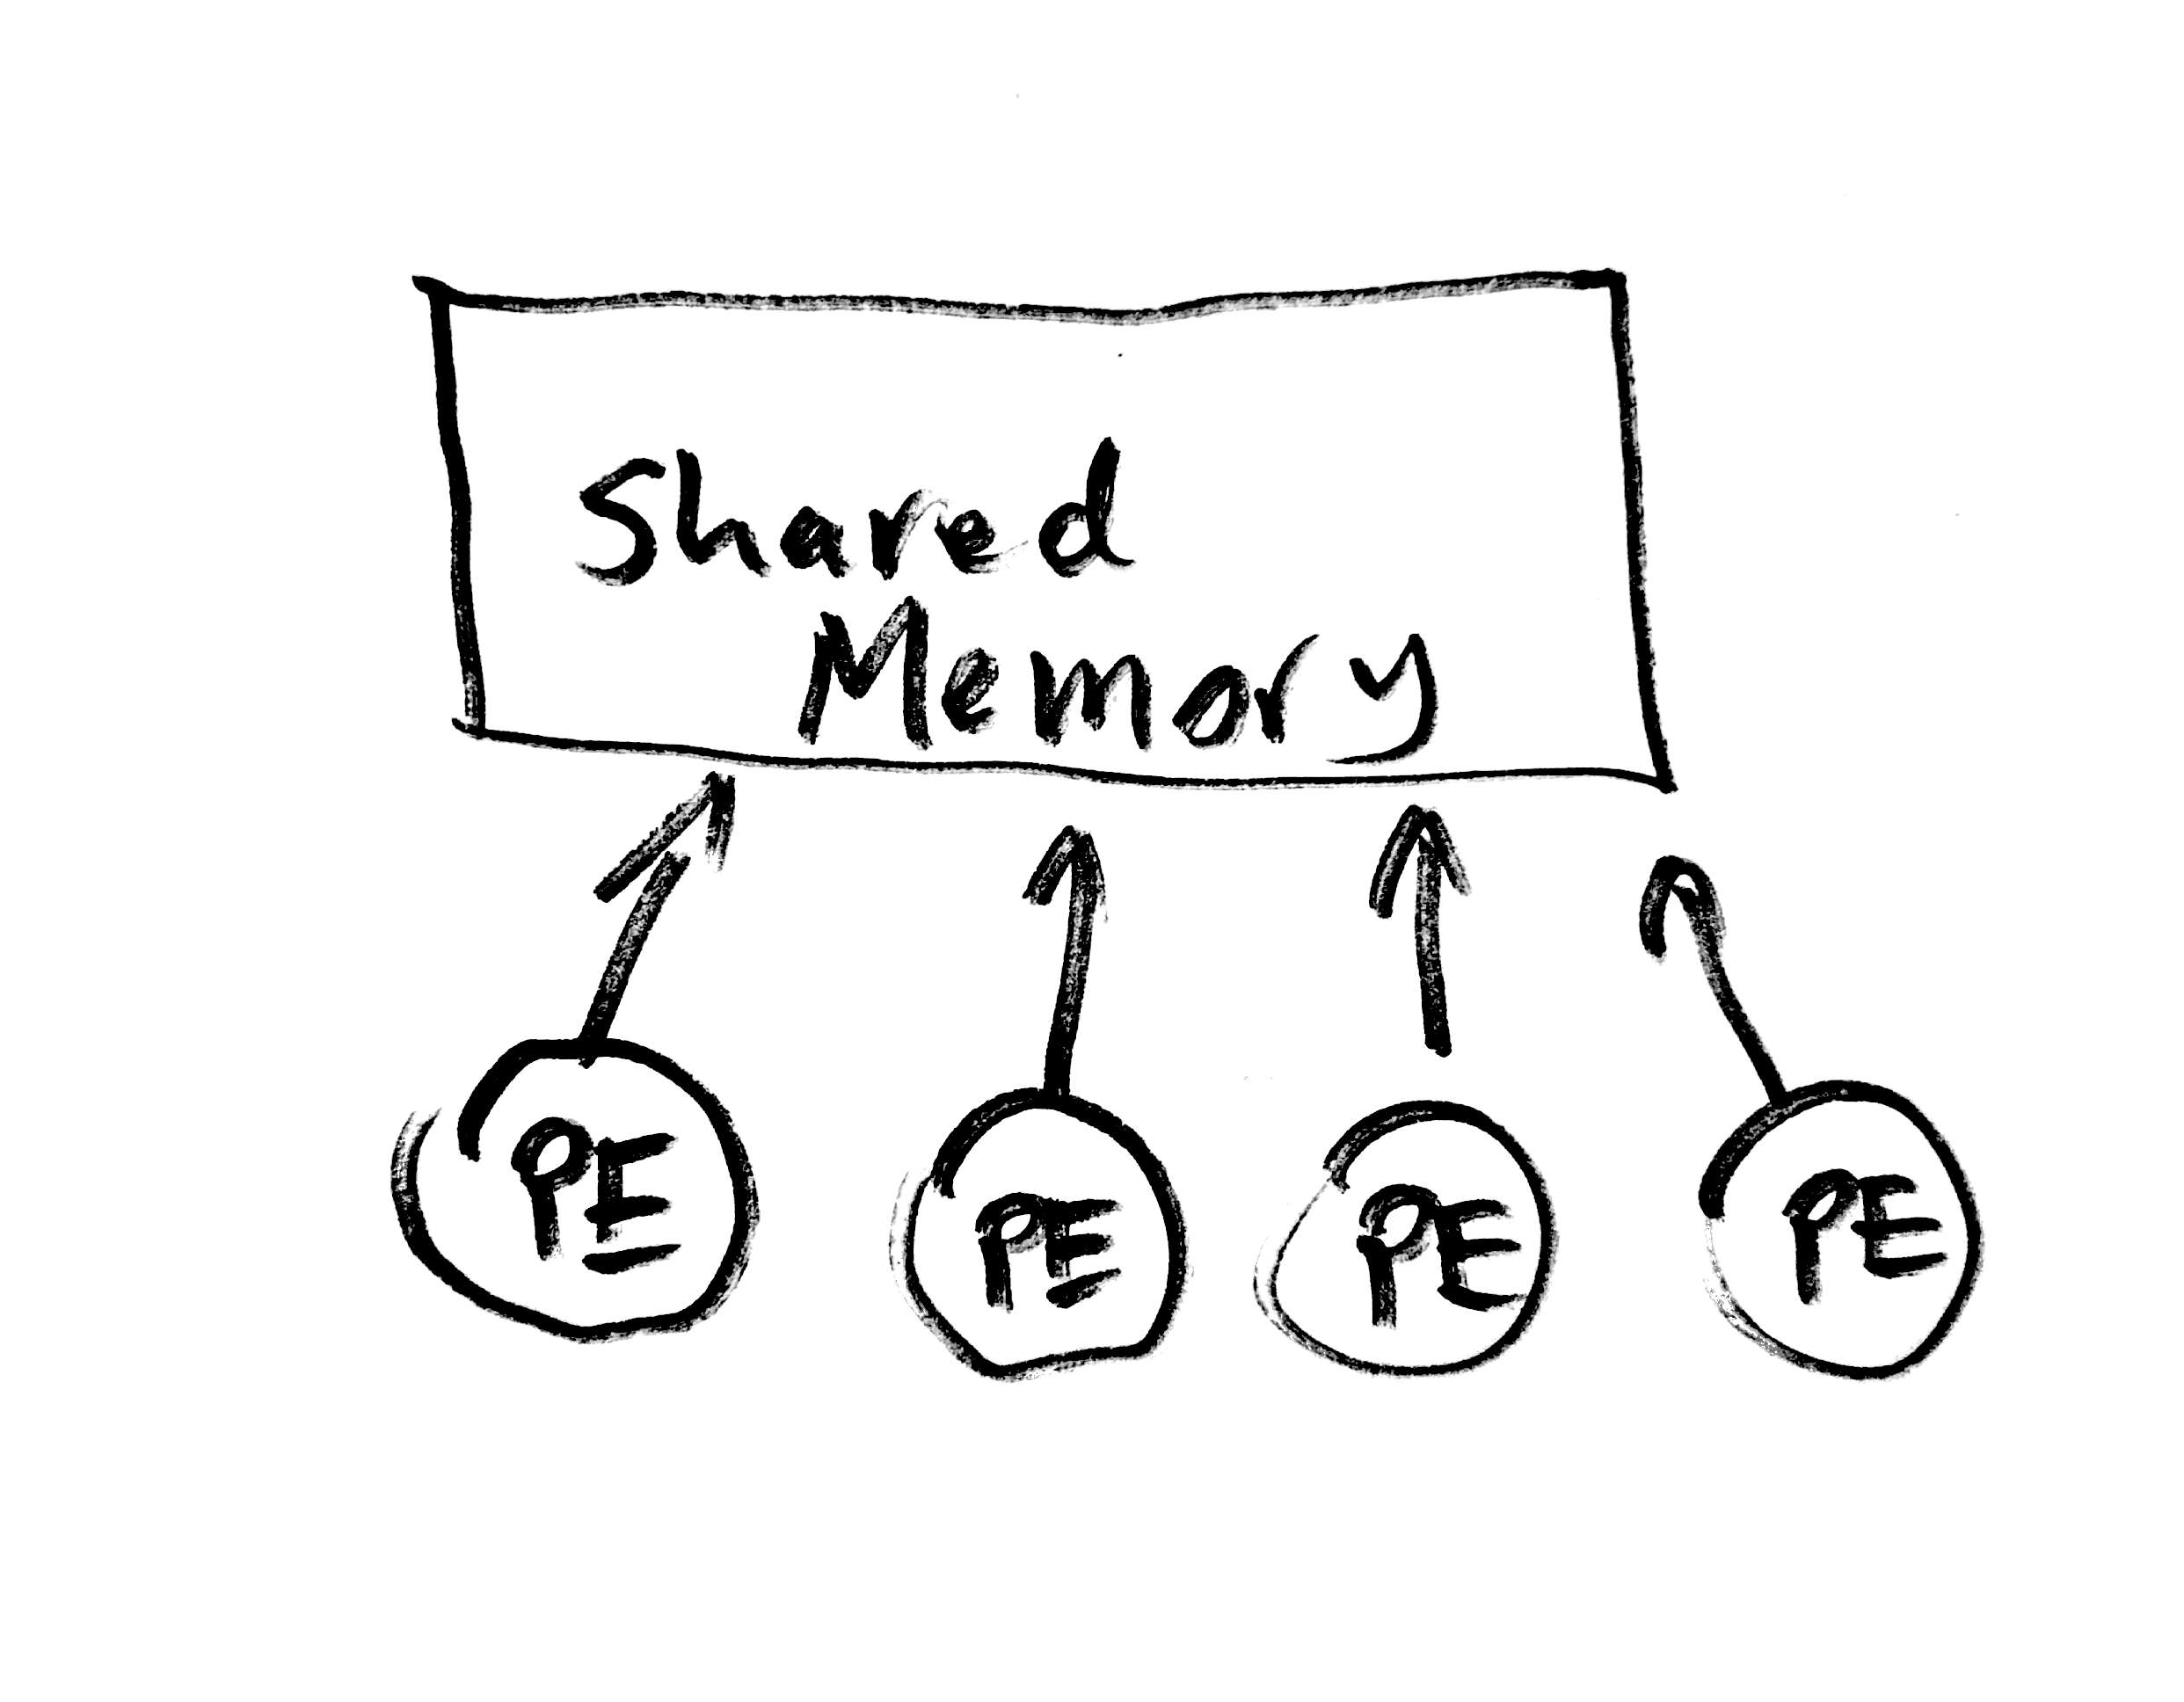
\includegraphics[width=0.75\textwidth]{pram}
  \caption{PRAM Model}
\end{figure}


\section{Max Element Algorithm}
Suppose we want to find the max element in a sequence or array.

\subsection{Naive Algorithm}
The naive approach is to just access each element 1 time sequentially computing the max.
This has the following time and work complexities, assuming all the numbers are unique:

$$T(N) = O(N)$$
$$W(N) = O(N)$$

\subsection{Binary Tree Algorithm}
But can we do better? Yes. If we treat the decision problem as a binary tree then we can get $logn$ time complexity. Note, this processes is similar to MapReduce. The basic idea is to divide and conquer. Here, the original list is assigned to a set of workers who make decisions which look like a binary tree. The root of this tree is the max value.

$$T(N) = O(logN)$$
$$W(N) = O(N)$$

Note, we cannot do better than $O(N)$ work complexity since we must visit all nodes. This is just common sense.
\subsection{Ludicrous Speed}
What about an algorithm using as many workers as possible to solve the task? Then we can embed the max value problem into a sort of dependency matrix.

$$T(N) = O(1)$$
$$W(N) = O(N^2)$$

\begin{algorithm}
    \begin{algorithmic}[]
	\State $\forall i, isBiggest[i] := 1$
        \ForAll{$i, j$}
	    \If{$A[j] > A[i]$}
            	\State $isBiggest[i] \gets 0$
	    \EndIf
        \EndFor
	\If{$isBiggest[i]$}
	   \State $MAX := A[i]$
	\EndIf
    \end{algorithmic}
    \caption{Ludicrous Speed Algorithm}
\end{algorithm}
\end{document}





